\par Dans cette partie nous allons ainsi vous présenter les trois briques logicielles réalisé pour ce projet et les méthodes de pré-traitement réalisés :

\begin{itemize}
	\item Pré-traitement : formatage des données
	\item Détermination du sentiment du tweet
	\item Détermination de l'opinion towards
	\item 
\end{itemize}

\section{Formatage des données}
\par Afin d'améliorer les performances des différents blocs de cette implémentation, nous avons choisi de formater au mieux les données. Uniquement les tweets sont concernés pas ce formatage.

\par Plusieurs méthodes ont été appliquées:
\begin{itemize}
  \item transformation en minuscule de tous les caractères en majuscule.
  \item suppression du hashag \#semst présent à la fin de chaque tweet, et n'apportant aucun caractère informatif au tweets.
  \item remplacement des symboles pouvant être exprimés par des mots en ledit mot. Par exemple, au symbole \% correspond le mot "percent", au symbole \& le mot "and", ...
  \item suppression de tous les symboles ne pouvant pas être exprimés pas des mots, en particulier les symboles de ponctuation.
  \item transformation des formes contractées en leur forme étendue. Par exemple, à "ma'am" correspond le mot "madam", à "I'm" les mots "I am".
  \item transformation des nombres en le mot "number". En effet, la valeur exprimée n'a pas d'influence sur le sens du tweet.
  \item transformation des mentions (utilisation du symbole @) d'utilisateurs, en le mot "someone". Dans certains contextes, la valeur de cette mention pourrait être intéressante (dans le cas ou on arriverait à déterminer si cette mention a une valeur positive ou non par exemple), mais de part l'implémentation que nous avons choisi, ce formatage est plus pertinent, et améliore l'apprentissage du bloc "Opinion towards" detection.
  \item transformation de tous les verbes en leur forme infinitive.
\end{itemize}

\par Quelques autres formatages des tweets pourraient être pertinents dans le cadre de ce projet:
\begin{itemize}
  \item si plusieurs mots ont un synonyme en commun, il pourrait s'avérer judicieux de remplacer lesdits mots par ce synonyme. Ainsi, nous réduisons le dictionnaire de mots utilisés, et pouvons améliorer l'apprentissage du bloc "Opinion towards" detection.
  \item il est compliqué d'extraire le sens des hashags utilisés dans les tweets, cependant il correspondent régulièrement à un groupe de mots collés. Ainsi un hashag comme \#NetNeutrality pourrait être décomposé en deux mots, "net" et "neutrality".
  \item transformation des mots au pluriel en leur forme au singulier. En effet, ils seront interprétés comme étant des mots différents par le bloc "Opinion towards" detection, alors qu'ils n'influent pas sur sens général du tweet.
  \item suppression des répétitions de mots.
\end{itemize}
Certains formatage appliqués ne sont pas forcément des plus précis, et pourraient être améliorés. Par exemple, dans le cas du remplacement des contractions en mots, il est difficile de déterminer si "he's" correspond à "he is" ou "he has".

\section{Sentiment analysis}

\section{"Opinion towards" detection}

\section{Stance detection}

La partie "Stance detection" consiste à déterminer l'opinion du tweet par rapport au sujet, c'est-à-dire si le tweet est "pour", "contre" ou "neutre" vis à vis du sujet. Cette étape prend en entrée le "Target" (le sujet), le "Sentiment" (positif, négatif ou autre) et l'"Opinion Towards" (le tweet donne un opinion par rapport au sujet, le tweet donne un opinion qui n'a pas de rapport avec le sujet, ou le tweet ne donne pas d'opinion). Ces deux derniers sont déterminés dans les étapes précédentes. Cette dernière étape est donc sensible aux taux d'erreur précédemment obtenus.
La combinaison de ces trois entrées permet de déterminer la "stance". \\

Cette partie est un problème de classification basique, qui prend en entrée trois paramètres qui renvoie une sortie. C'est un problème de classification multi-classe, en effet la sortie se compose de 3 classes : "FAVOR", "AGAINST" et "NONE". \\

\subsection{POC - Traitement des données}

Une première approche a été de tester différentes méthodes de classification usuelles comme SVM et bayes.

Pour cela, un petit traitement sur les données s'impose, effectivement pour utiliser de telles méthodes il est d'abord nécessaire de labelliser les données avec des classes numérotées pour s'abstraire des chaînes de caractères. \\
Dans le jeu de données de train fourni, il y 5 "target" différents, en ce qui concerne le "sentiment" il y a 3 classes possibles et il en est de même pour l'"opinion towards".

En essayant de réaliser une SVM, nous nous sommes rendu compte que dans le jeu de données de test il y avait maintenant 6 "target". En effet, les tweets concernant le sujet "Donald Trump" ont été ajouté. Or, le modèle ne peut pas fonctionner pour un sujet qui n'a pas été appris. 
La solution a dont été de fusionner les ensembles d'apprentissage et de test et de les redécouper de manière aléatoire afin d'obtenir des tweets de l'ensemble des "target" dans l'ensemble d'apprentissage.

\subsection{POC - Test de méthodes de classification}

Tout d'abord, nous avions décidé d'implémenter une méthode de classification bayésienne et une méthode SVM, ensuite il a également été possible d'implémenter d'autres méthodes classification.

Pour un premier test, toutes les méthodes ont été testées avec les paramètres par défaut, et renvoient les taux d'erreurs suivants :
\begin{itemize}
\item Bayes avec un noyau Gaussien : 31,74$\%$
\item SVM Linéaire : 37,62$\%$
\item SVM : 33,11$\%$
\item K plus proches voisins : 34,47$\%$
%\item Arbre de décision : 24,49$\%$
\end{itemize}

Les résultats de ce POC sont disponibles dans la section \hyperref[annexe-stance-detection]{Annexe : POC - Find Stance} p.2-3.

\subsection{POC - Test de paramètres de la méthode SVM}

Ensuite, il s'est avéré intéressant de tester différents paramètres de la méthode SVM. Le résultat est présent sur la figure suivante.

\begin{figure}[!h]
\centering
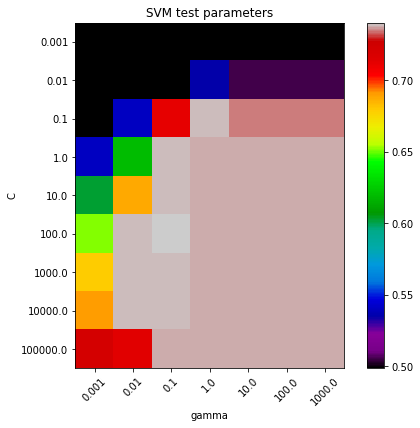
\includegraphics{src/annexes/POC_FindStance_V2/output_24_0.png}
\end{figure}

\textbf{Les valeurs C=100 et gamma=0.1 ont donc été choisi pour réaliser cette SVM, qui fournit finalement un taux d'erreur de $24,49\%$}.

\subsection{Implémentation d'une SVM}

%TODO





